\section{Meal schedule}

The two figures in this section, \cref{MealScheduleList} and \cref{MealScheduleBar}, displays two design ideas for the meal schedule aspect of the program. In \cref{MealScheduleList} 2 sketches are shown, and they indicate the first idea that were thought of in the context of design. The left sketch show the meal schedule for a week, and the right show the meals scheduled on a specific day. In \cref{MealScheduleBar} the screen that is going to be the design of the program is shown. The sketches of \cref{MealScheduleList} have been combined to make the final sketch shown in \cref{MealScheduleBar}

\begin{figure}[H]
	\centering
    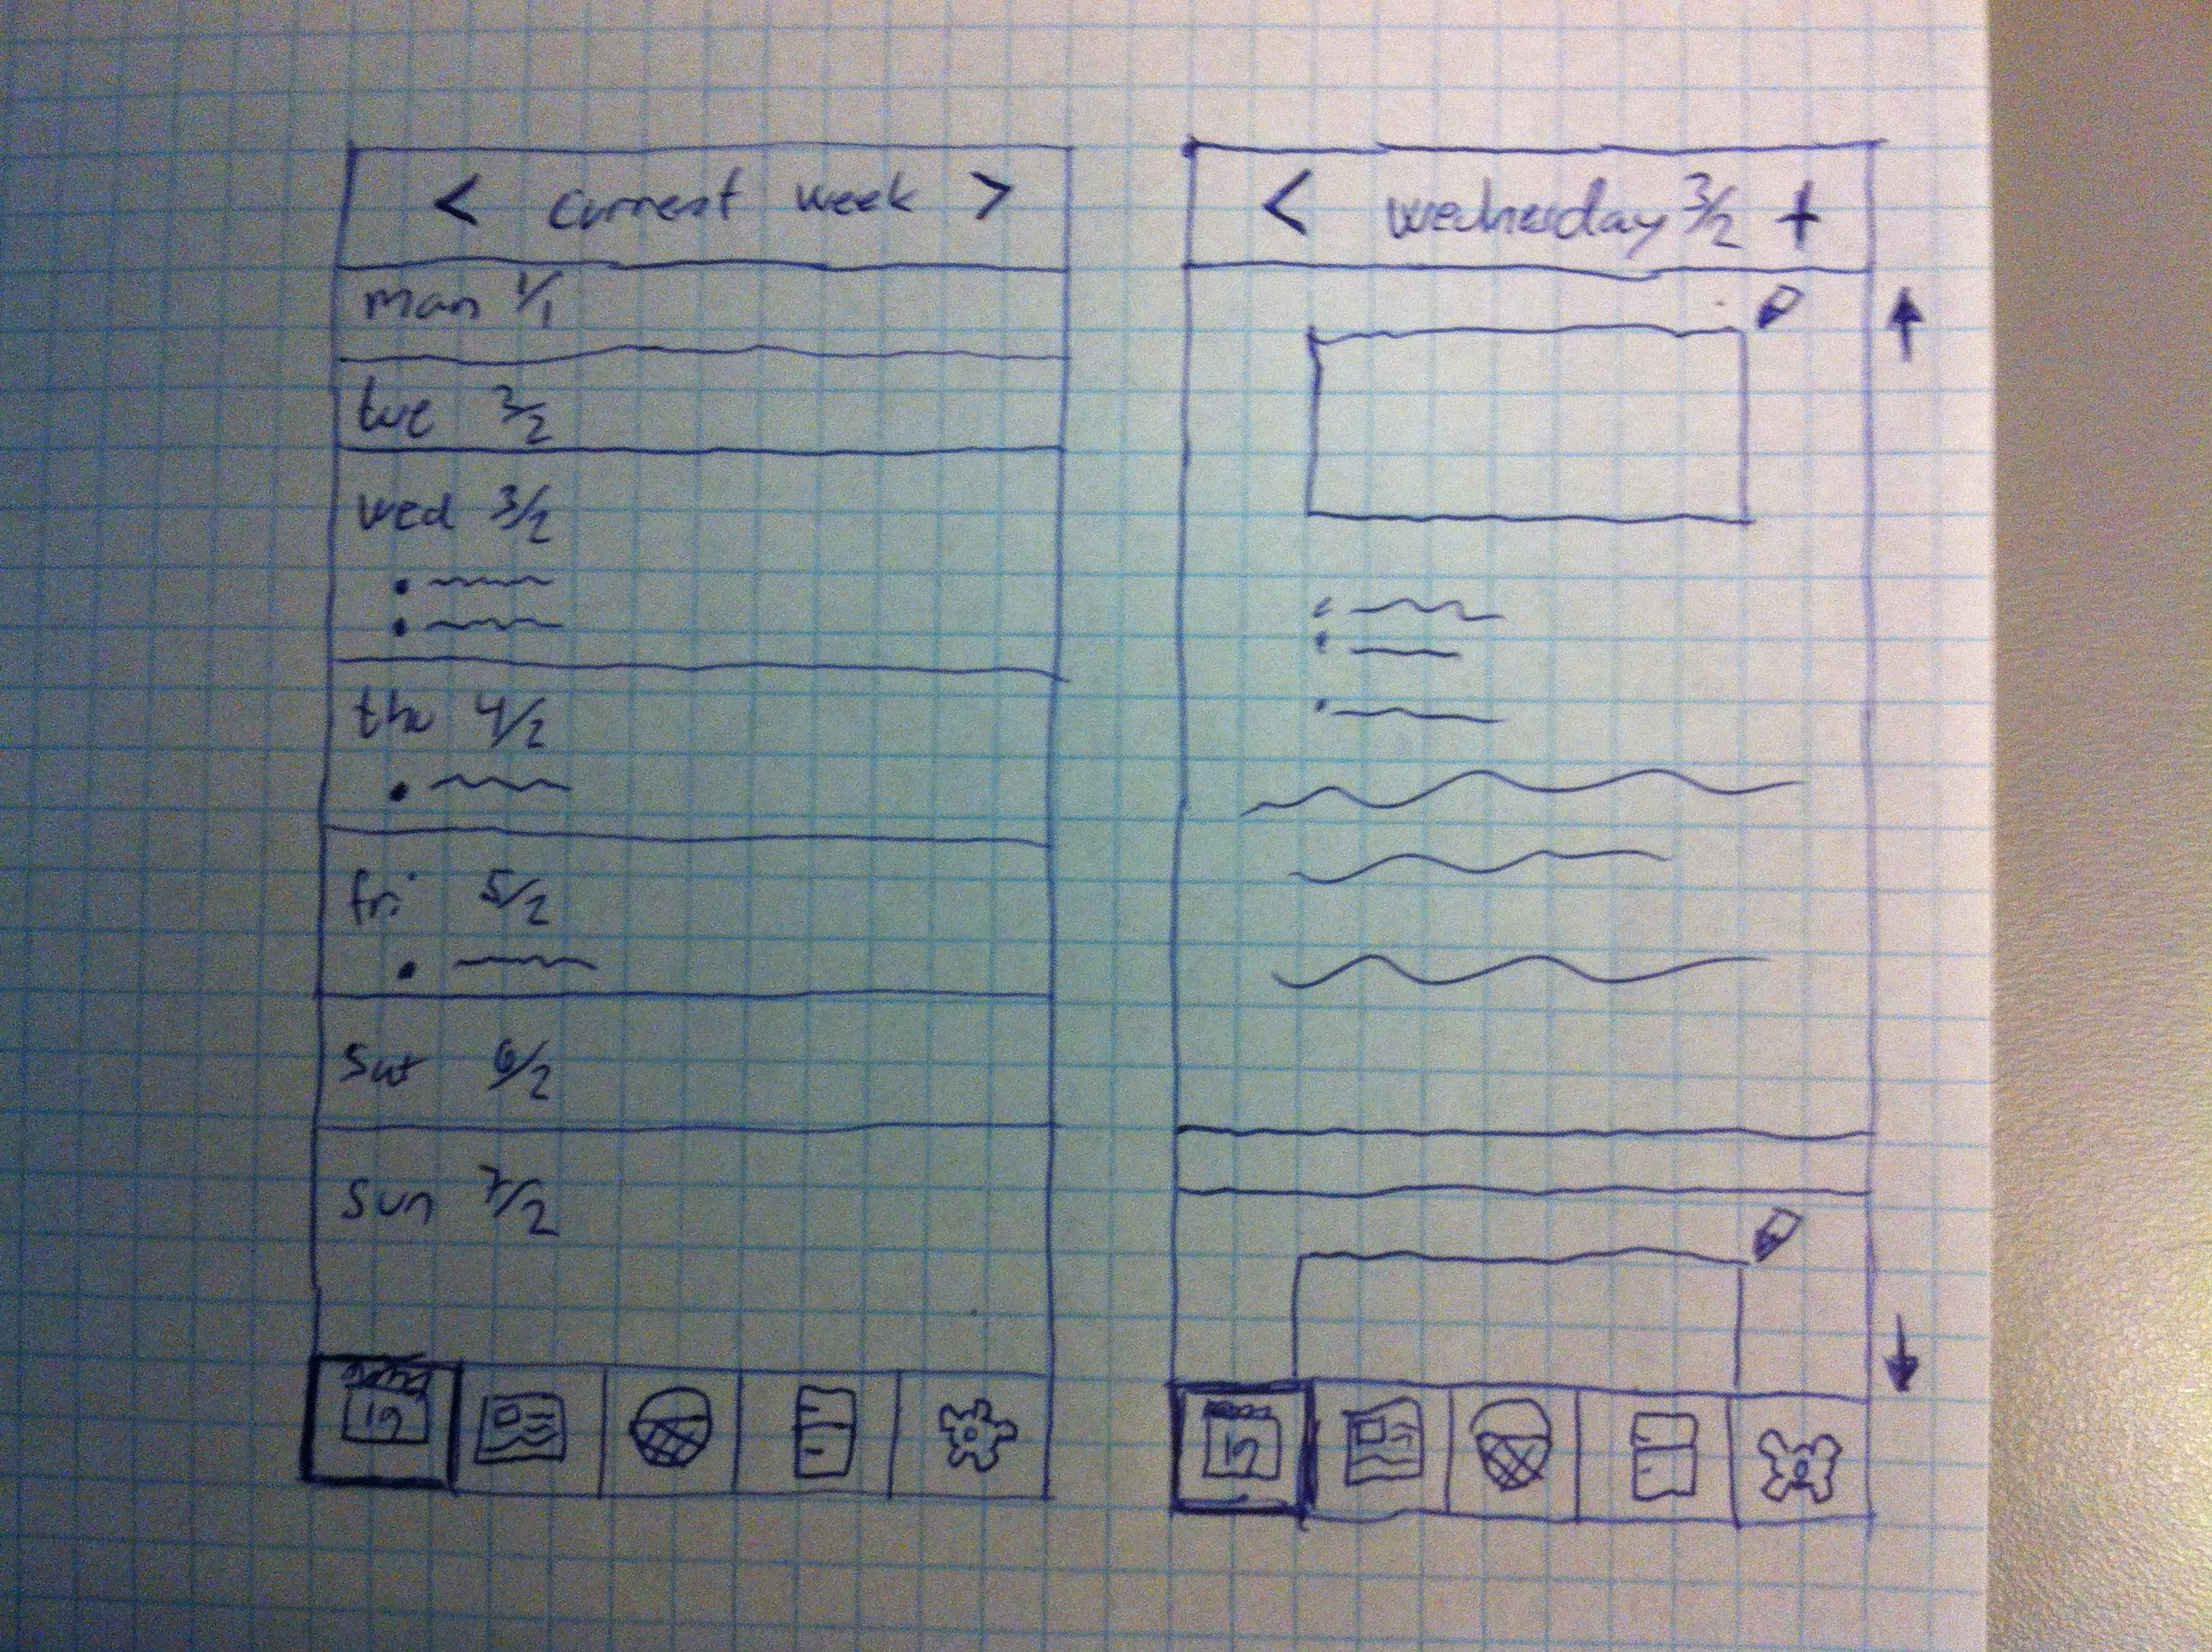
\includegraphics[width=0.5\textwidth]{Grafik/FoodPlanner/FinalMealScheduleSketch1}
	\caption{The left screen shows 7 days of a specific week and the right screen shows scheduled meals on a specific day.}
	\label{MealScheduleList}
\end{figure}

\subsection{First draft: Week schedule}

Looking at the first draft of the week schedule, \cref{MealScheduleList}, there are two elements to look at:

\begin{itemize}
    \item Navigation bar
    \item Schedule
\end{itemize}

The navigation is placed at the top of the screen, because the sides of a screen, and especially top and bottom, are places that users tend to look to find navigation, and since the bottom is already used by the navigation of the entire program, it is the natural choice to place it at the top. This also gives some symmetry to the program, because as mentioned, the bottom is filled by the navigation bar for the entire program.

The schedule element of the sketch, shows seven days of the schedule. Seven is chosen because it is a week, and the availability to plan a week ahead is useful if the user plans the same day of the week, and plans the rest of the weeks. Each day of the schedule would show the name of the recipe scheduled, the date of the day, and some of the ingredients needed in the recipe. If the user chose to click a day, the day would expand, and more information about the scheduled meal would appear.

\subsection{First draft: Specific recipe screen}

The specific recipe screen

\subsection{Final design}


Beginning with the screen to the left on \cref{MealScheduleList} there are three areas of concern. In the middle of the screen there is a list overview of 7 days. Each day shows the name, date, ingredients that the user has of scheduled meals on a specific day. If there are many meals scheduled the list will expand to outside of the screen view. The user can scroll to view all days and press a specific day to view details about it. This method of display gives the user an easy and informative view of the week days. The top bar is used to navigate between weeks. The right screen on \cref{MealScheduleList} displays the screen for a specific day. The navigation bar on the bottom is unchanged. On the middle there are an overview of all the planned recipes which the user can scroll through. On each of the recipe there is a icon for the user to change a specific meal. The meals will display information such as ingredients, title, number of participant. The top bar has a button to add meals to the specific day and it also shows what day it is and an arrow for the user to navigate back to the week overview.  

\begin{figure}[H]
	\centering
    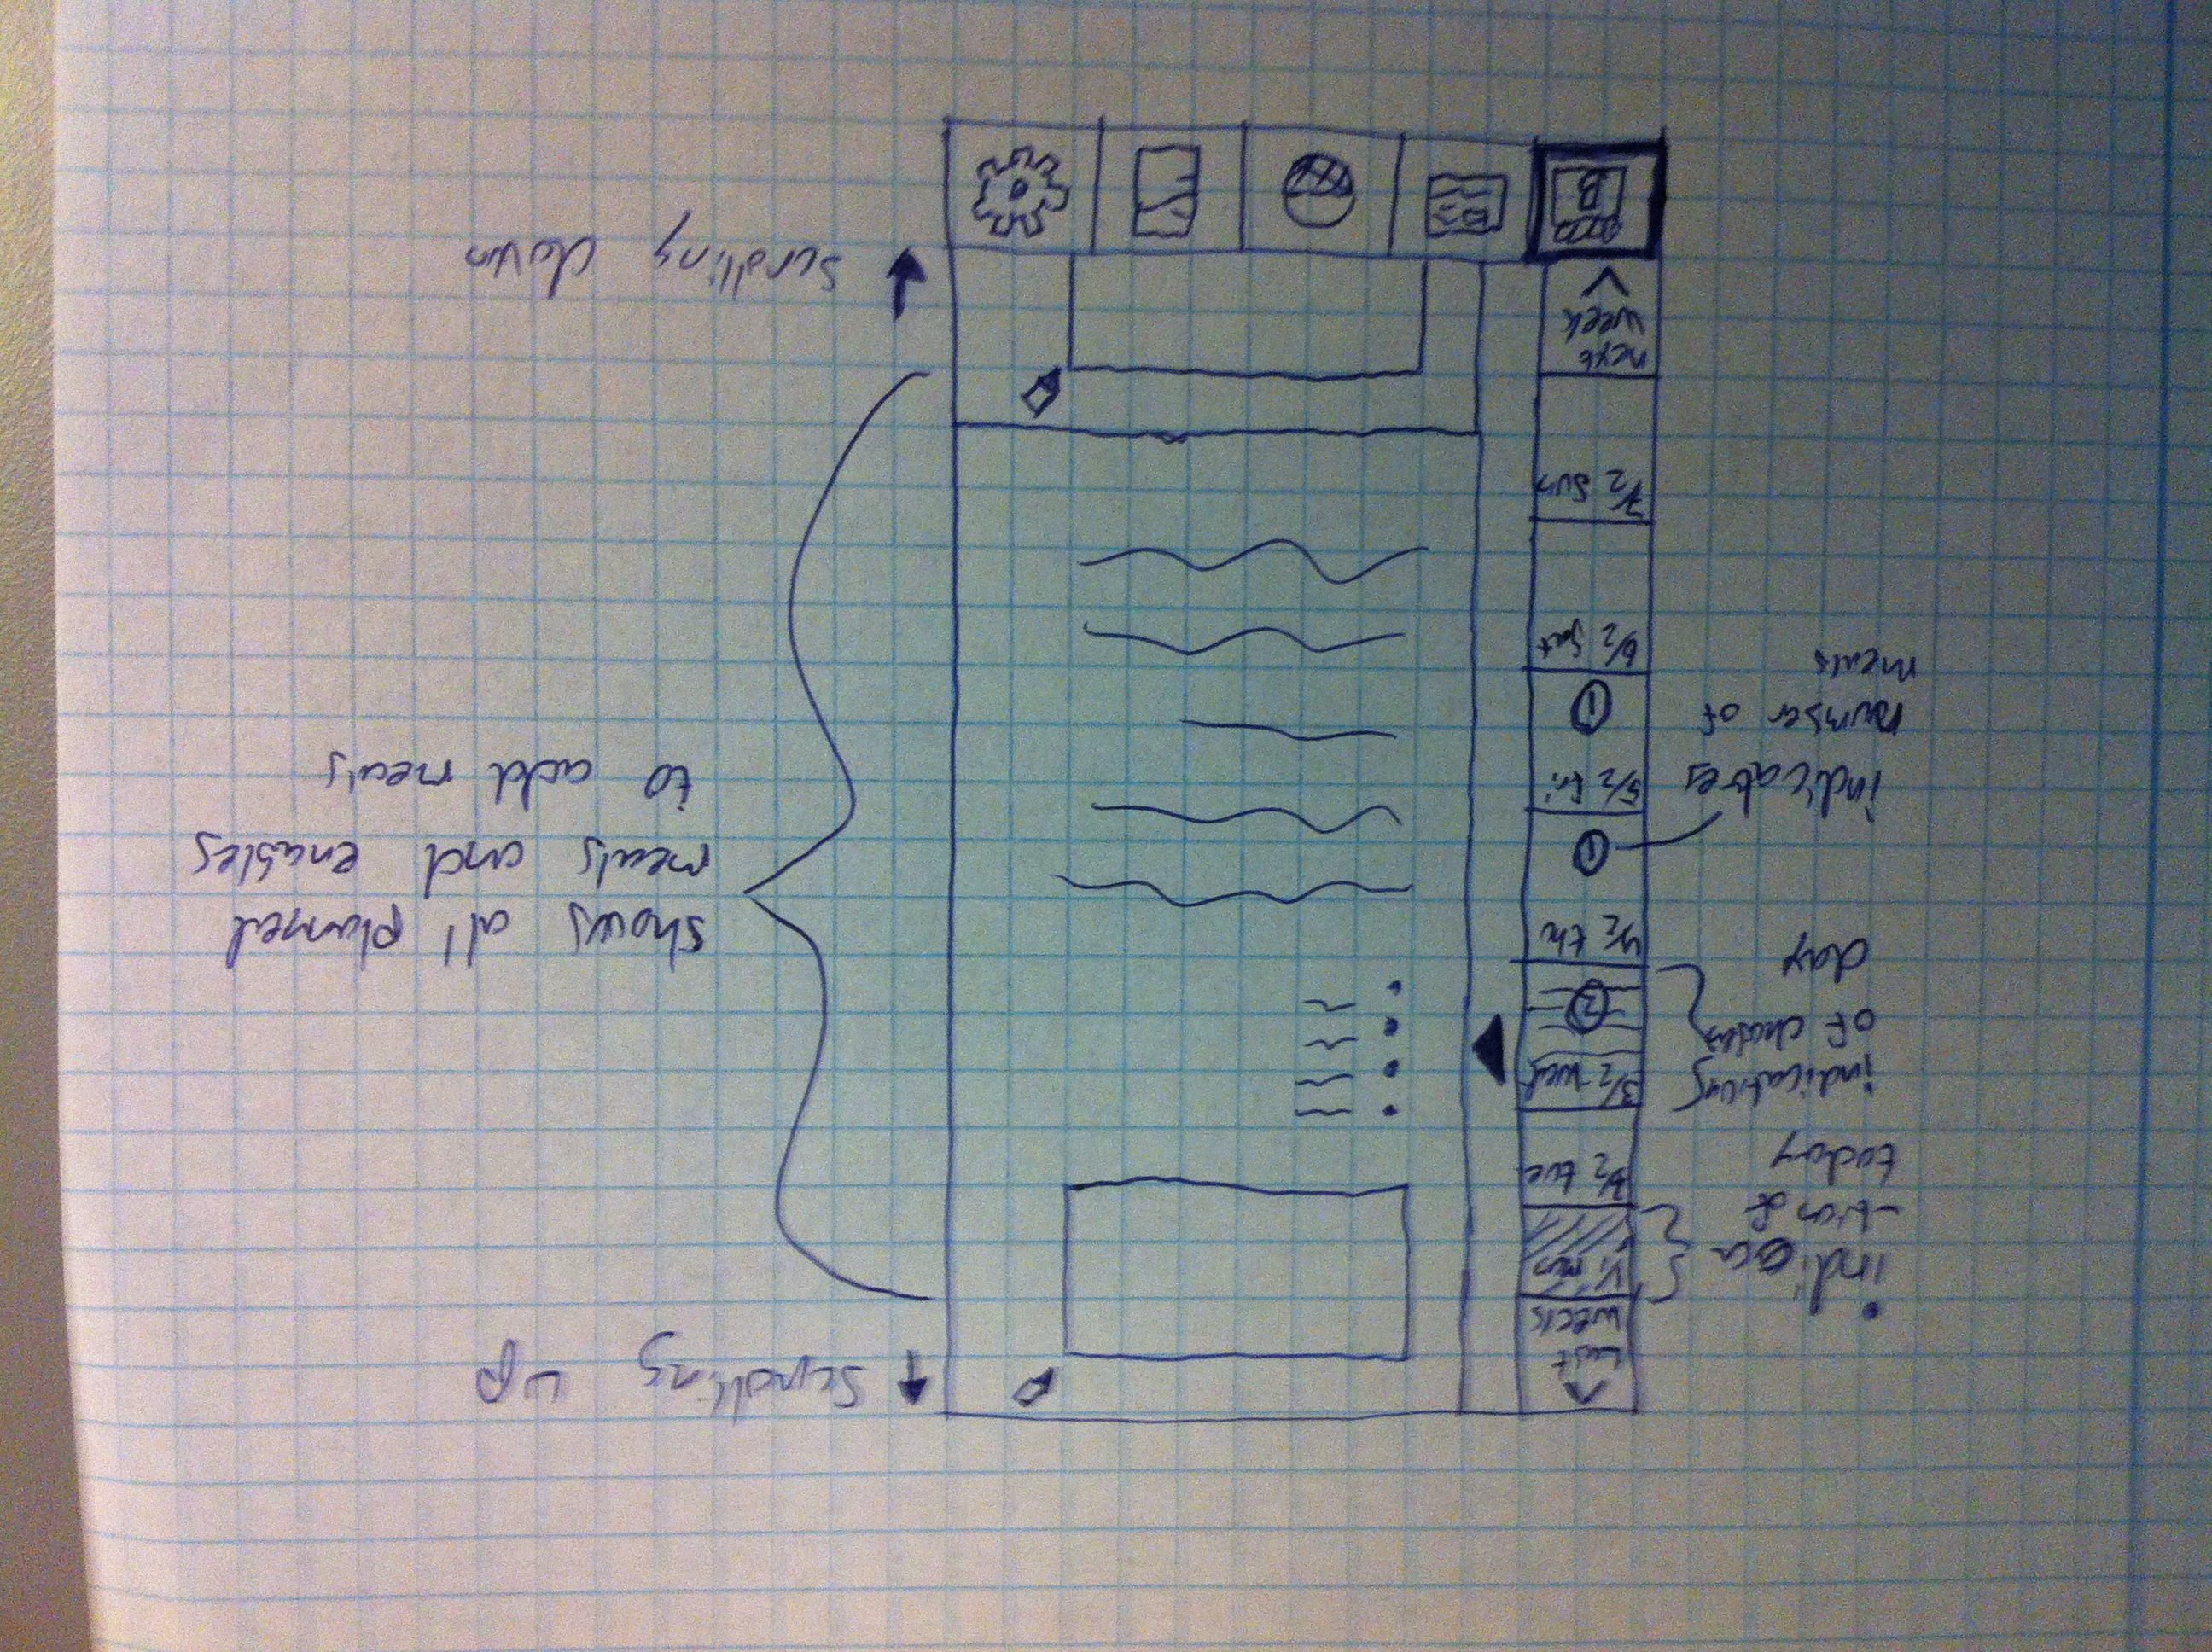
\includegraphics[width=0.5\textwidth]{Grafik/FoodPlanner/FinalMealScheduleSketch2}
	\caption{This sketch merges both of the screens above into one screen with the weeks on the left bar and the scheduled meals as a list on the right side of the screen.}
	\label{MealScheduleBar}
\end{figure}

On \cref{MealScheduleList} there a displayed a different approach to the design of the meal schedule. This screen has a weekly overview on the left bar. At the top and bottom of this bar there are buttons to navigate between weeks. Each day on this bar has a title, date and a indication of the number of scheduled meals. There are also an indication of the current day and the day that has been selected. On  the left side of the screen there is an overview of the scheduled meals just as the method used on the right screen on \cref{MealScheduleList}. 

